% comment out for student version
\ifdefined\Student\relax\else\def\Teacher{}\fi

\documentclass[12pt]{article}

\title{Data Types}
\author{Chris Mayfield and Stoney Jackson}
\date{Summer 2021}

%\ProvidesPackage{cspogil}

% fonts
\usepackage[utf8]{inputenc}
\usepackage[T1]{fontenc}
\usepackage{mathpazo}

% spacing
\usepackage[margin=2cm]{geometry}
\renewcommand{\arraystretch}{1.4}
\setlength{\parindent}{0pt}

% orphans and widows
\clubpenalty=10000
\widowpenalty=10000
\pagestyle{empty}

% figures and tables
\usepackage{graphicx}
\usepackage{multicol}
\usepackage{tabularx}
\usepackage{wrapfig}

% fixed-width columns
\usepackage{array}
\newcolumntype{L}[1]{>{\raggedright\let\newline\\\arraybackslash\hspace{0pt}}m{#1}}
\newcolumntype{C}[1]{>{\centering\let\newline\\\arraybackslash\hspace{0pt}}m{#1}}
\newcolumntype{R}[1]{>{\raggedleft\let\newline\\\arraybackslash\hspace{0pt}}m{#1}}

% include paths
\makeatletter
\def\input@path{{Models/}{../../Models/}}
\graphicspath{{Models/}{../../Models/}}
\makeatother

% colors
\usepackage[svgnames,table]{xcolor}
\definecolor{bgcolor}{HTML}{FAFAFA}
\definecolor{comment}{HTML}{007C00}
\definecolor{keyword}{HTML}{0000FF}
\definecolor{strings}{HTML}{B20000}

% table headers
\newcommand{\tr}{\bf\cellcolor{Yellow!10}}

% syntax highlighting
\usepackage{textcomp}
\usepackage{listings}
\lstset{
    basicstyle=\ttfamily\color{black},
    backgroundcolor=\color{bgcolor},
    numberstyle=\scriptsize\color{comment},
    commentstyle=\color{comment},
    keywordstyle=\color{keyword},
    stringstyle=\color{strings},
    columns=fullflexible,
    keepspaces=true,
    showlines=true,
    showstringspaces=false,
    upquote=true
}

% code environments
\newcommand{\java}[1]{\lstinline[language=java]{#1}}%[
\lstnewenvironment{javalst}{\lstset{language=java,backgroundcolor=}}{}
\lstnewenvironment{javabox}{\lstset{language=java,frame=single,numbers=left}\quote}{\endquote}

% PDF properties
\usepackage[pdftex]{hyperref}
\urlstyle{same}
\makeatletter
\hypersetup{
  pdftitle={\@title},
  pdfauthor={\@author},
  pdfsubject={\@date},
  pdfkeywords={},
  bookmarksopen=false,
  colorlinks=true,
  citecolor=black,
  filecolor=black,
  linkcolor=black,
  urlcolor=blue
}
\makeatother

% titles
\makeatletter
\renewcommand{\maketitle}{\begin{center}\LARGE\@title\end{center}}
\makeatother

% boxes [optional height]
\newcommand{\emptybox}[1][10em]{
\vspace{1em}
\begin{tabularx}{\linewidth}{|X|}
\hline\\[#1]\hline
\end{tabularx}}

% models
\newcommand{\model}[1]{\section{#1}\nopagebreak}
\renewcommand{\thesection}{Model~\arabic{section}}

% questions
\newcommand{\quest}[1]{\subsection*{Questions~ (#1)}}
\newcounter{question}
\newcommand{\Q}{\vspace{1em}\refstepcounter{question}\arabic{question}.~ }
\renewcommand{\thequestion}{\#\arabic{question}}

% sub-question lists
\usepackage{enumitem}
\setenumerate[1]{label=\alph*)}
\setlist{itemsep=1em,after=\vspace{1ex}}

% inline answers
\definecolor{answers}{HTML}{C0C0C0}
\newcommand{\ans}[1]{%
\ifdefined\Student
    \leavevmode\phantom{~~\textcolor{answers}{#1}}
\else
    ~~\textcolor{answers}{#1}
\fi}

% longer answers [optional height]
\newsavebox{\ansbox}
\newenvironment{answer}[1][4em]{
\nopagebreak
\begin{lrbox}{\ansbox}
\begin{minipage}[t][#1]{\linewidth}
\color{answers}
}{
\end{minipage}
\end{lrbox}
\ifdefined\Student
    \phantom{\usebox{\ansbox}}%
\else
    \usebox{\ansbox}%
\fi}


\begin{document}

\maketitle

Java supports two main types of data: \emph{primitive types} like \java{int} and \java{double} that represent a single value, and \emph{reference types} like \java{String} and \java{Scanner} that represent more complex data.

\rolenames

\guide{
  \item Explain how using roles improves the team's success.
  \item Name Java's primitive data types and give examples of each one.
  \item Identify illegal assignment statements, and explain why they are illegal.
  \item Describe what it means for variables to store a reference to an object.
}{
  \item Providing feedback on how well other team members are working. (Teamwork)
}{
The meta activity reinforces the importance of roles.
Successful teams are able to accomplish all the tasks outlined on the \github{Handouts/role-cards-mayfield.pdf}{Role Cards}, and there's too many things for one person to keep track.
Ask the reflectors to pay special attention to their role during today's activity, and invite them at some point to report to share what they have observed.

On \ref{literals}, students may struggle with letters used in primitive values (i.e., F and L).
Rather than just say what everything means, direct students back to \ref{primitive-types.tex} and have them read out loud the type names.
%Explain that \texttt{float} is a floating-point data type, and ask students to guess where the name \texttt{double} comes from.
\ref{allowed} is good for report-out, allowing students to collectively develop a rule for when an assignment is allowed.
The solution files \sol{Act03}{Assign1.java} and \sol{Act03}{Assign2.java} are available for demonstration.
When reporting out, introduce the term \emph{literal}.

%It might be helpful to have a couple of examples handy to challenge their assumptions.
%But be careful, examples like \texttt{short x = 3; byte y = 3; char c = 3;} may open a can of worms.
%If these issues come up, you'll need to explain that \texttt{javac} will check the range of the value, and if it is acceptable, allow the assignment (i.e., \texttt{byte z = 255;} will fail).

\ref{reference-types.tex} introduces a technique for drawing memory diagrams to show the difference between primitive and reference types.
On \ref{twostrs}, have multiple teams draw their diagrams on the board.
Address misconceptions that arise (e.g., drawing multiple string objects).
It might be helpful at this point to direct students to \href{https://cscircles.cemc.uwaterloo.ca/java_visualize/}{Java Visualizer}, which draws similar diagrams.
Select the option ``Show String/Integer/etc objects, not just values'' for it to display references as arrows.

Key questions: \ref{allowed}, \ref{varval}, \ref{twostrs}

Source files: \src{Act03}{TaylorSwift.java}
}

\model{Team Disruptions}
% Based on Model 4 of "We Are a Learning Team!" by Urik Halliday

Common disruptions to learning in teams include:
  talking about topics that are off-task,
  teammates answering questions on their own,
  entire teams working alone,
  limited or no communication between teammates,
  arguing or being disrespectful,
  rushing to complete the activity,
  not being an active teammate,
  not coming to a consensus about an answer,
  writing incomplete answers or explanations,
  ignoring ideas from one or more teammates.


\quest{10 min}


\Q Pick four of the disruptions listed above.
For each one, find something from the role cards that could help improve the team's success.
Use a different role for each disruption.

\begin{enumerate}[itemsep=1ex]

\item Manager:

\begin{answer}[2em]
limited communication between teammates
\end{answer}

\item Presenter:

\begin{answer}[2em]
ignoring ideas from one or more teammates
\end{answer}

\item Recorder:

\begin{answer}[2em]
writing incomplete answers or explanations
\end{answer}

\item Reflector:

\begin{answer}[2em]
teammates answering questions on their own
\end{answer}

\end{enumerate}

\begin{center}
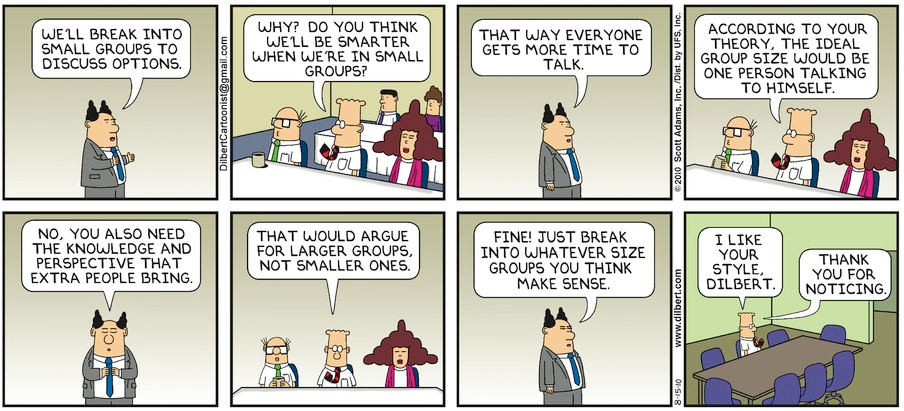
\includegraphics[height=2.85in]{disrupt1.png}
% see http://www.amureprints.com/reprints/classroom
\par \itshape \footnotesize
Dilbert by Scott Adams.
\copyright\ Andrews McMeel Syndication.
\url{http://dilbert.com/strip/2010-08-15}
\end{center}

\newpage
\model{Primitive Types}
\label{CS1/primitive-types}

\vspace{-1ex}
\begin{table}[h!]
\begin{tabularx}{\linewidth}{|X|X|X|X|}
\hline
\tr Keyword    & \tr Size & \tr Min Value & \tr Max Value \\
\hline
\java{byte}    & 1 byte   & $-128$    & $127$ \\
\hline
\java{short}   & 2 bytes  & $-32,768$ & $32,767$ \\
\hline
\java{int}     & 4 bytes  & $-2^{31}$ & $2^{31}-1$ \\
\hline
\java{long}    & 8 bytes  & $-2^{63}$ & $2^{63}-1$ \\
\hline
\java{float}   & 4 bytes  & $\pm 3.4 \times 10^{-38}$  & $\pm 3.4 \times 10^{38}$ \\
\hline
\java{double}  & 8 bytes  & $\pm 1.7 \times 10^{-308}$ & $\pm 1.7 \times 10^{308}$ \\
\hline
\java{boolean} & N/A      & \java{false}     & \java{true} \\
\hline
\java{char}    & 2 bytes  & \java{'\\u0000'} & \java{'\\uffff'} \\
\hline
\end{tabularx}
\end{table}

Note that 1 byte is 8 bits, i.e., eight ``ones and zeros'' in computer memory.
Since there are only two options for each bit, with 8 bits you can represent $2^8 = 256$ possible values.


\quest{10 min}


\Q Which of the primitive types are integers? Which are floating-point? Which are not numeric?

\begin{answer}
\end{answer}


\Q Why do primitive types have ranges of values? What determines the range of the data type?

\begin{answer}
\end{answer}


\Q Why can't computers represent every possible number in mathematics? Will they ever be able to do so?

\begin{answer}
\end{answer}


\Q Since a \java{byte} can represent 256 different numbers, why is its max value 127 and not 128?

\begin{answer}
\end{answer}


\Q What is the data type for each of the following values?

\begin{quote}
\begin{multicols}{2}
1.14159 \ans{double} \\[1ex]
0       \ans{int} \\[1ex]
-1.0F   \ans{float} \\[1ex]
123     \ans{int}

7.2E-4  \ans{double} \\[1ex]
0.0     \ans{double} \\[1ex]
-13L    \ans{long} \\[1ex]
'0'     \ans{char}
\end{multicols}
\end{quote}


\Q Given the following variable declarations, which of the assignments are not allowed?

\begin{quote}
\begin{multicols}{2}

\begin{javalst}
byte miles;
short minutes;
int checking;
long days;
float total;
double sum;
boolean flag;
char letter;
\end{javalst}

\begin{javalst}
checking = 56000;
total = 0;
sum = total;
total = sum;
checking = miles;
sum = checking;
sum = days;
days = "0";
\end{javalst}

\end{multicols}
\end{quote}


\Q \label{allow} In general, when does Java allow you to assign one type of numeric variable to another?

\begin{answer}
\end{answer}


\Q Based on your answer to \ref{allow}, list all possible assignments in this format:
\java{int} $\gets$ \java{short}

\begin{answer}
\end{answer}

\newpage
\model{Reference Types}

\begin{quote}
\begin{minipage}{0.5\linewidth}

\begin{javalst}
int count;
double price;
String name;
Scanner in;

count = 0;
price = 1.99;
name = "Beyonce";
in = new Scanner(System.in);
\end{javalst}

\end{minipage}
\begin{minipage}{0.5\linewidth}

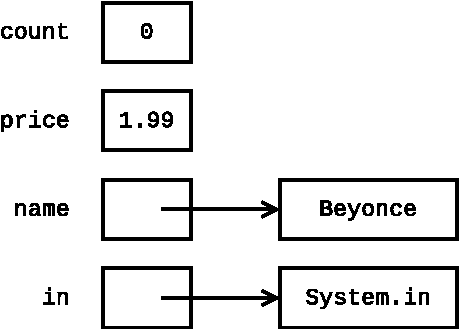
\includegraphics{CS1/reference1.pdf}

\end{minipage}
\end{quote}

Java has eight primitive types (see \ref{CS1/primitive-types}).
All other types of data are called \emph{reference} types, because \textbf{their value is a memory address}.
When drawing memory diagrams, use an arrow to \emph{reference} other memory locations (rather than make up integer values for the actual addresses).


\quest{10 min}


\Q What are the reference types in the example above?

\begin{answer}
\end{answer}


\Q In terms of style, what is the difference between primitive and reference type names?

\begin{answer}
\end{answer}


\Q Variables in Java can use at most eight bytes of memory. Explain why the values for Beyonce and System.in cannot be stored directly in the memory cells for \java{name} and \java{in}.

\begin{answer}
\end{answer}


\Q What is the value of the variable \java{count}? What is the value of the variable \java{price}?

\begin{answer}
\end{answer}


\Q What is the value of the variable \java{name}? What is the value of the variable \java{in}?

\begin{answer}
\end{answer}


\Q \label{assign} Carefully explain what it means to assign one variable to another. For example, what does the statement ~ \java{price = count;}~ do in terms of memory?

\begin{answer}
\end{answer}


\Q Draw a memory diagram for the following code. Make sure your answer is consistent with what you wrote for \ref{assign}.

\begin{javalst}
int width;
float score;
String first;
Scanner input;
String other;

width = 20;
score = 0.94;
first = "Taylor";
input = new Scanner(System.in);
score = width;
other = first;
\end{javalst}


\end{document}
